\section{C5: cell pooling is not a super-graph}
\label{sec:pooled}

C5 concatenates live article-cells across the eight 8-node topologies.
That operation is a table union.
It is not a physical 64-node graph, and it is not the 63-node D-net custom topology.
\Cref{fig:c5pool} shows the four instrument-by-arm headlines on the concatenated set.

\begin{figure}[t]
\centering
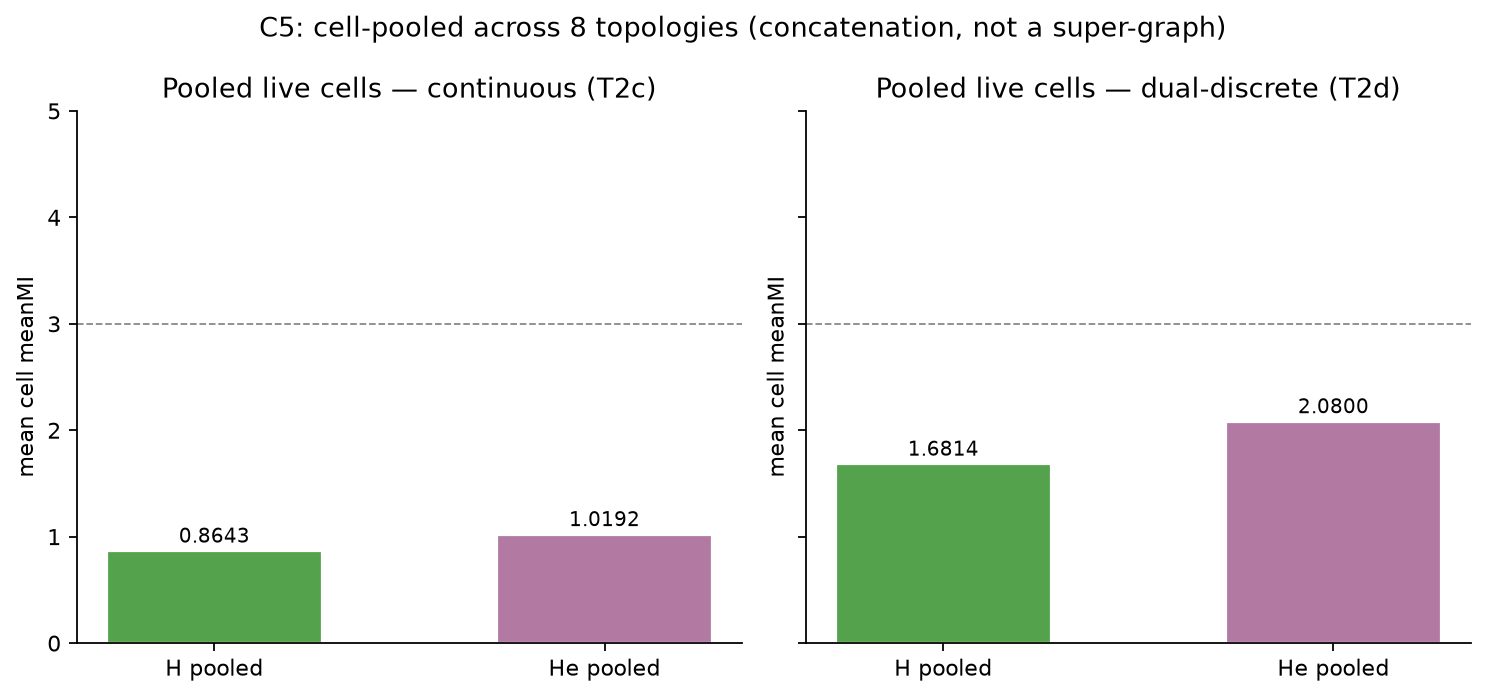
\includegraphics[width=\textwidth]{figures/fig06_c5_pooled_h_vs_he.png}
\caption[C5 cell-pooled H vs He]{C5: cell-pooled H versus He on concatenated live rows.
Pooling is not a super-graph.
$N=1$.
Source: \texttt{fig06\_c5\_pooled\_h\_vs\_he.png}.}
\label{fig:c5pool}
\end{figure}

On the concatenated set, He still exceeds H on both instruments (continuous $\Delta=0.1549$; dual-discrete $\Delta=0.3986$).
Topology-equal weighting does not flip the sign (\Cref{tab:c5w,tab:c5pool}).
The sign is compatible with conspiracy composition, not with a buffering law.

T2c family mean \MI{} on pooled H cells is conspiracy $2.2194$, climate action $0.1729$, science/environment $0.1118$.
T2d family means are conspiracy $3.1691$, climate action $1.0488$, science/environment $0.8687$.
On pooled He cells, \texttt{mix\_00} (four conspiracy) is T2c $1.7712$ versus \texttt{mix\_02} (zero conspiracy) $0.2645$; T2d \texttt{mix\_00} is $3.1321$ versus \texttt{mix\_02} $1.1882$.
Restricting H to the conspiracy family reverses the naive H/He story: conspiracy H sits well above overall He.
\Cref{fig:c5comp} records that composition split.

\begin{figure}[t]
\centering
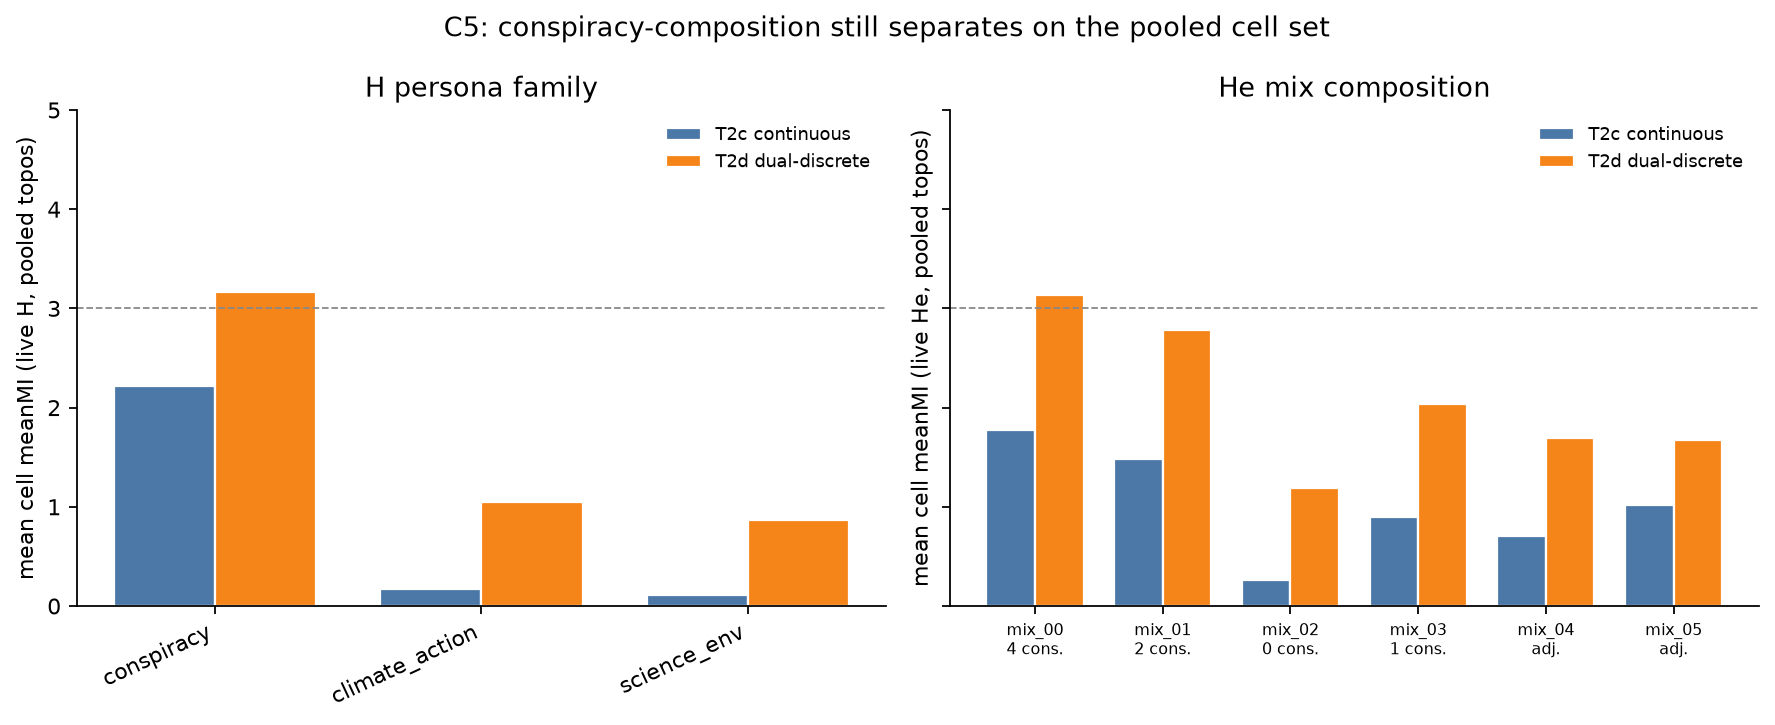
\includegraphics[width=\textwidth]{figures/fig07_c5_conspiracy_composition.png}
\caption[C5 conspiracy composition]{C5: family means on pooled H cells and mix means on pooled He cells.
Conspiracy remains the high group on both instruments.
$N=1$.
Source: \texttt{fig07\_c5\_conspiracy\_composition.png}.}
\label{fig:c5comp}
\end{figure}

\begin{table}[t]
\centering
\caption[C5 concatenated live-cell pools]{C5 concatenated live-cell pools.
These rows are table unions, not a 64-node graph and not D-net.}
\label{tab:c5pool}
\scriptsize
\begin{tabular}{lrrrr}
\toprule
Pool & $n$ live & meanMI & meanNodeMPR & \kstar{} rate \\
\midrule
T2c\_H all topologies & 480 & 0.8643 & 0.8630 & 14.2\% \\
T2c\_He all topologies & 238 & 1.0192 & 1.0140 & 7.6\% \\
T2d\_H all topologies & 478 & 1.6814 & 1.6839 & 20.1\% \\
T2d\_He all topologies & 240 & 2.0800 & 2.0737 & 32.1\% \\
T2c\_H conspiracy family & 168 & 2.2194 & 2.2145 & 40.5\% \\
T2c\_H science/env.\ family & 195 & 0.1118 & 0.1130 & 0.0\% \\
T2c\_H climate-action family & 117 & 0.1729 & 0.1724 & 0.0\% \\
T2d\_H conspiracy family & 159 & 3.1691 & 3.1799 & 59.7\% \\
T2c\_He mix\_00/\_01 (conspiracy-heavy) & 80 & 1.6204 & 1.5921 & 11.2\% \\
T2c\_He mix\_02 (conspiracy-free) & 41 & 0.2645 & 0.2648 & 0.0\% \\
\bottomrule
\end{tabular}
\end{table}

\begin{table}[t]
\centering
\caption[C5 cell-pooled versus topology-equal]{C5: cell-pooled versus topology-equal H/He means.
Neither column is a super-graph.}
\label{tab:c5w}
\begin{tabular}{lrrrrrr}
\toprule
Contrast & Pooled H & Pooled He & $\Delta$ & Topo-eq.\ H & Topo-eq.\ He & $\Delta$ \\
\midrule
T2c H vs He & 0.8643 & 1.0192 & 0.1549 & 0.8630 & 1.0356 & 0.1725 \\
T2d H vs He & 1.6814 & 2.0800 & 0.3986 & 1.6832 & 2.0806 & 0.3974 \\
\bottomrule
\end{tabular}
\end{table}

\paragraph{Invalid extra pools.}
Averaging discrete with continuous H still has no auditor ($(0.8643+1.6814)/2=1.2729$).
Averaging H with He inside one instrument still hides composition.
D-net rows are not concatenated into \Cref{tab:c5w}.
Section~\ref{sec:dnet} treats the 63-node custom graph as a separate object.
